\section{Ensemble Methods}
\begin{itemize}
    \item Suppose we have many different weak models (better than random)
    \item Get prediction from all of them and take a vote
    \item Class with most votes is the predicted class
    \item Commonly used towards the end of a project
    \item \textcolor{blue}{Requirement} enough models / diverse models
\end{itemize}

\textbf{Wisdom of Crowd}
\begin{itemize}
    \item Suppose you have a difficult question
    \item Ask many people and aggregate the answer
    \item This might work very well instead of finding the best suited person
\end{itemize}

\textbf{Transfer}
\begin{itemize}
    \item Wisdom of Crowd can be applied to ML
    \item Instead of finding the best model, aggregate the results of weak models
    \item Aggregate predictions of regressors or classifiers
    \item Might get better accuracy than the best predictor
    \item Ensemble: group of predictors
\end{itemize}

\textbf{Aggregate predictions}
\begin{itemize}
    \item \textcolor{blue}{Hard voting} Predict class with most votes
    \item \textcolor{blue}{Soft voting} Predict class with the highest class probability
\end{itemize}


\subsection{Bagging and Pasting}
\textbf{Bagging (Bootstrap Aggregating)}
\begin{itemize}
    \item Sampling with replacement (a data point can be selected more than once)
    \item Allows data points to be used several times
\end{itemize}
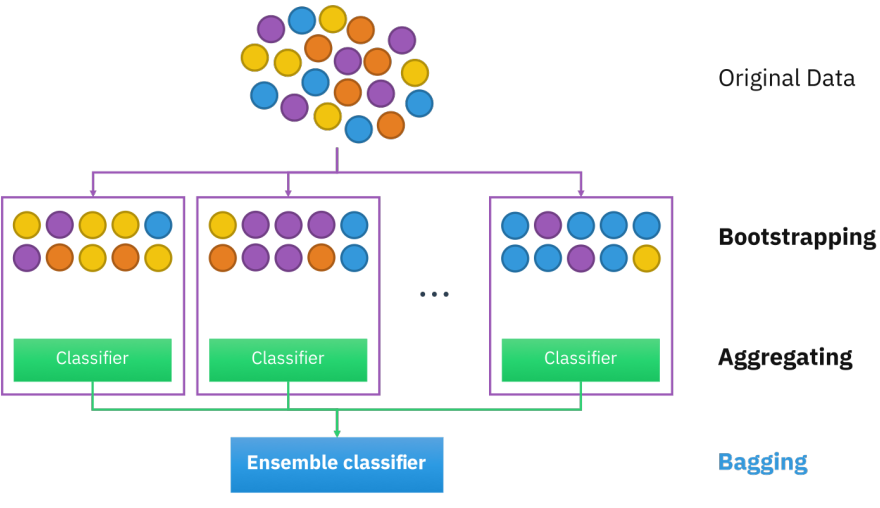
\includegraphics[width=0.5\linewidth]{bagging.png}
\textbf{Pasting}
\begin{itemize}
    \item Sampling without replacement (a data point can be selected only once)
\end{itemize}

\subsection{No free lunch theorem}
\textit{No single machine learning algorithm is universally the best-performing algorithm for all problems}

\begin{itemize}
    \item No single algorithm will solve all your machine learning problems better than every other algorithm.
    \item Make sure you completely understand a machine learning problem and the data involved before selecting an algorithm to use.
    \item All models are only as good as the assumptions that they were created with and the data that was used to train them.
    \item Simpler models like logistic regression have more bias and tend to underfit, while more complex models like neural networks have more variance and tend to overfit.
    \item The best models for a given problem are somewhere in the middle of the two bias-variance extremes.
    \item To find a good model for a problem, you may have to try different models and compare them using a robust cross-validation strategy.
\end{itemize}

\textbf{Out of Bag (oob) Evaluation}
\begin{itemize}
    \item Using Bagging
    \item Some Data Points may not be used at all
    \item Use them for evaluation
\end{itemize}
